

\documentclass[a4paper]{article}
\setlength{\textwidth}{15cm}
\setlength{\evensidemargin}{0cm}
\setlength{\oddsidemargin}{1cm}
\usepackage{hyperref}
\usepackage{alltt}
\usepackage{graphicx}
\usepackage{listings}


\begin{document}

\section{SMIYang}
\label{sec:smiyang}

\lstset{numbers=left, numberstyle=\tiny, stepnumber=1, numbersep=5pt}
\lstset{escapeinside={(*@}{@*)}}

\subsection{Presentation}


It is  common in the  network management world  that a protocol  and a
data model are  separated even if jointly designed,  as it was already
the case in the  SNMP\cite{rfc1157} protocol and its SMI\cite{rfc1442}
data   modeling,CO\-PS\cite{rfc2748}   and  SP\-PI\cite{rfc3159},   or
SMI\-ng and  various protocols \cite{rfc3780}  (GDMO and CMIS  or WBEM
and CIM outside the IETF scope).

NETCONF\  \cite{rfc4741} is the  IETF standard  that emerged  from the
netconf   working   group   to   configure   network   devices.    The
netmod\footnote{http://www.ietf.org/html.charters/netmod-charter.html}
working group  defines YANG \cite{yang01}  as a candidate  language to
specify  data  models  of  values  carried by  NETCONF.   This  report
describes a YANG parser called {\sl jYang\/}\ that provides a syntaxic
and  semantic validation  of  YANG specifications  (called modules  or
sub-modules).

A YANG\  specification contains formal definitions of  data types that
will  model   real  data   maintained  by  NETCONF\   agents.   Formal
definitions follow  the YANG\  syntax. YANG\ provides  constructs that
give  semantics to XML  data that  are exanged  by NETCONF  agents and
managers.  As an  XML document is a collection  of imbricated markups,
YANG\ defines  statements that  can be mapped  on pattern  of markups.
Moreover  YANG\  allows  reusability  of specifications  with  generic
statements or augmentation/extension statements.\\

Following is an example of  a part of a YANG specification\footnote{All
example in  this report are  inspired from the  draft\cite{yang01}} that
describes  a table  of network  interfaces, a  conceptual view  of two
entries and the XML document of this configuration:\\


\noindent
\begin{center}
\begin{tabular}{lcl}
\begin{minipage}{.20\textwidth}
\begin{verbatim}
list interfaces {
   key index;
   leaf index {
     type int8;
   }
   leaf name {
     type string;
   }
   leaf type {
     type string;
   }
   leaf speed {
     type int64;
   }
}
\end{verbatim}
\end{minipage}
&
\begin{minipage}{.42\textwidth}
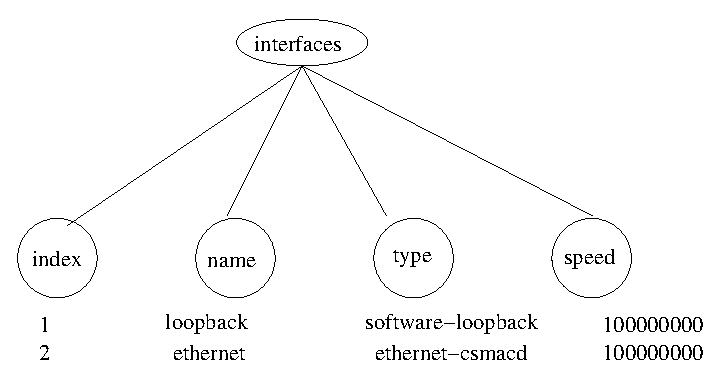
\includegraphics[scale=.6]{listinterface.eps}
\end{minipage}
&
\begin{minipage}{.2\textwidth}
\begin{small}
\begin{verbatim}
<list>
  <index>
     1
  </index>
  <name>
     loopback
  </name>
  <type>
     software-loopback
  </type>
  <speed>
     100000000
  </speed>
  <index>
     2
  </index>
  <name>
     ethernet
  </name>
  <type>
     ethernet-csmacd
  </type>
  <speed>
     100000000
  </speed>
</list>
\end{verbatim}
\end{small}
\end{minipage}
\end{tabular}
\end{center}

YANG\ specifications are organized in modules and submodules
that contain data type definitions and operation descriptions. 


YIN is  an alternative XML-based syntax for  YANG\ specifications. YIN
specifications   can   be   generated   from  YANG\   ones   and   are
equivalent.  The goal  of  YIN specifications  is  to enable  seemless
interactions with  XML based tools  (as XSLT).  {\sl  jYang\/}\ parser
allows the generation of YIN specifications from YANG.

\section{{\sl jYang\/}}

{\sl  jYang\/}\ is  a  java  parser for  YANG\  specifications and  an
application  programming interface offering  a programmatic  access in
java to YANG\ specifications.

\subsection{YANG\ Parser}

The    java    parser    is    built   with    JJTree    and    JavaCC
\footnote{https://javacc.dev.java.net}  but  no  external  library  is
needed to use it.

\begin{itemize}
\item
lexical and syntax  checks are conformant to the  ABNF grammar given in
\cite{yang01}
\item
semantical check covers following features :
\begin{itemize}
\item
name scoping and accessibility for typedef, grouping, extension, uses,
leaf and  leaflist, inside  a module  or submodule  and with  imported and
included specifications.
\item
type restriction  for any type (integer,  boolean, bits, float,\ldots)
and typedef
\item
default value and restriction
\item
augment existing node
\item
Xpath for schema node in augment, leaf (of key ref type) and list (for
unique statement)
\end{itemize}
\end{itemize}

\subsection{Repository}

{\sl jYang\/}\ is  an open source distribution  of our toolkit  under the GPL
licence. The official repository is at the INRIA Gforge web site :\\
\begin{verbatim}
http://jyang.gforge.inria.fr
\end{verbatim}

\subsection{{\sl jYang\/}\ tools}

\subsubsection{{\sl jYang\/}\ parser use}

{\sl jYang\/}\ is distributed  as a java jar file  called {\tt jyang.jar} and
configured to be executable. The synoptic is :

\begin{verbatim}
java -jar jyang.jar [-h] [-f format] [-o outputfile] [-p paths] file [file]*
\end{verbatim}

\begin{itemize}
\item
{\tt -h} print the synoptic
\item
{\tt  -f format}  specifies the  format for  a translated  output (yin
format for example)
\item
{\tt -o outputfile} the name of the translated output (standard output
if not given) ignored if no format are given
\item
{\tt -p  paths} a path where  to find other YANG\  specifications. It is
needed   if  import  or   include  statements   are  in   the  checked
specification or  if the environement variable {\tt  YANG\_PATH} is not
set.
\item
{\tt file  [file]*} specifies  files containing YANG\  specification. It
must be  one specification ({\tt  module} or {\tt submodule}  for each
file).
\end{itemize}

\paragraph{Errors}

Errors  in YANG\  specifications  are printed  on  the standard  error
output.   {\sl  jYang\/}\  stops  checking  at the  first  lexical  or
syntaxical error  but can find  more than one semantical  error.  When
such an error  is detected, the current bloc  statement is escaped and
{\sl jYang\/}\ passes to the next statement.

\subsubsection{Programmatic access}

{\sl  jYang\/}\ provides java  classes and  interfaces to  parse YANG\
specification inside a java  program. Internal representation of those
specifications can be  accessed throught the API defined  in the INRIA
technical report \cite{}. Below is an  example of how to parse a YANG\
specification.

\begin{lstlisting}
import java.io.*;
import jyang.*;

public class JyangTest {

   /**
   * Simple jyang test, parses and checks one YANG specification.
   * Imported or included modules or submodules are looked in the 
   * current directory.
   * Error messages are on the standard output
   * 
   * @param args YANG file name
   */
   public static void main(String[] args) throws Exception {
        FileInputStream yangfile = new FileInputStream(args[0]);(*@\label{getyangfile}@*)
        new yang(yangfile);(*@\label{jyangparser}@*)
        YANG_Specification spec = yang.Start();(*@\label{startjyang}@*)
        spec.check();(*@\label{jyangcheck}@*)
   }
}
\end{lstlisting}

The   program  first  gets   the  YANG\   specification  file   at  line
\ref{getyangfile}.    A    new   jyang   parser    is   created   line
\ref{jyangparser} with this file.  The lexical and syntactic check are
processed  at line  \ref{startjyang} and  return  a YANG\_specification
object  instance  that  can   be  semantically  checked,  as  at  line
\ref{jyangcheck}.



\subsection{Impact}

The {\sl jYang\/}  parser and the yang API have an  impact on the work
of the netmod  working group as they are  existing implementation of a
standard draft.   The parser can be  used by NETCONF  data modelers in
order to validate  their models.  The API allows  the developpement of
several backends as  html or xml.  {\sl jYang\/} can  be a support for
educational  purpose in  master or  engeneering  network configuration
teatching modules.


\subsection{Progress Report}

The java  code has a  size of about  15000 lines of code  (without the
generated code by JJTree and JavaCC) and has an executable size of 500
Ko. It was successfully  tested with several YANG specifications found
on      YANG     related     site      (www.netconfcentral.com     and
www.yang-central.org).

\subsection{Conclusion}

A YANG parser is achieved and an API allows YANG specification access
from java programs. Current works are on the new draft version
\cite{yang02} and a python backend that will be integrated in the
NETCONF python implementation called ENSUITE
framework\cite{CRIDLIG:2005:INRIA-00000804:1}.


\bibliographystyle{plain}
\bibliography{emanicsJyang}



\end{document}

